% !TEX root = HDA_MDRL.tex

\section{Results}
\label{sec:results}

\begin{table}[]
	\begin{tabular}{lccccc}
		\textbf{Task A}				& S1	& S2	& S3	& [S2 S3]	& S4	\\
									&		&		&		&			&		\\
		F1-measure (with Null class)&		& 		&		&			& 		\\
		Baseline					& 0.85	& 0.86	& 0.83	& 0.85		& 0.77	\\
		Contributed					& -		& 0.85	& 0.81	& 0.83 		& - 	\\
		Our results					& 0.91	& 0.76	& 0.83	& 0.88		& 0.79	\\
									&		&		&		&			&		\\
		F1-measure (no Null class)	&		&		&		&			&		\\
		Baseline					& 0.86	& 0.86	& 0.85	& 0.85		& 0.76	\\
		Contributed					& -		& 0.90	& 0.87	& 0.87 		& - 	\\
		Our results					& 0.94	& 0.78	& 0.90	& 0.84		& 0.89	\\
	\end{tabular}
	\caption{Comparison of results on modes of locomotion (task A), with and without the \textit{Null} class. For each of the baseline, contributed and our models, here are reported only the best scores achieved.}
	\label{tab:res_A}
\end{table}
\begin{table}[]
	\begin{tabular}{lccccc}
		\textbf{Task B}				& S1	& S2	& S3	& [S2 S3]	& S4	\\
									&		&		&		&			&		\\
		F1-measure (with Null class)&		& 		&		&			& 		\\
		Baseline					& 0.85	& 0.89	& 0.86	& 0.87		& 0.88	\\
		Contributed					& -		& 0.88	& 0.87	& 0.88 		& 0.71 	\\
		Our results					& 0.89	& 0.81	& 0.88	& 0.84		& 0.85	\\
									&		&		&		&			&		\\
		F-measure (no Null class)	&		&		&		&			&		\\
		Baseline					& 0.55	& 0.53	& 0.58	& 0.56		& 0.48	\\
		Contributed					& -		& 0.72	& 0.80	& 0.77 		& 0.17 	\\
		Our results					& 0.81	& 0.40	& 0.82	& 0.64		& 0.70	\\
	\end{tabular}
	\caption{Comparison of results on gesture recognition (task B), with and without the \textit{Null} class. For each of the baseline, contributed and our models, here are reported only the best scores achieved.}
	\label{tab:res_B}
\end{table}

As in most of the works mentioned in section \ref{sec:related_work}, besides accuracy, we used $F_1$ measure to estimate the goodness of our models. Defining precision and recall as: 
\begin{equation}
	p = \frac{TP}{TP+FP} \qquad r = \frac{TP}{TP+FN}
\end{equation}
where \textit{TP = true positives}, \textit{FP = false positives} and \textit{FN = false negatives}, the $F_1$ measure is evaluated as the harmonic average between the two. In particular, since we deal with a multi-class problem we need to add a measure of weight to the $F_1$ equation:
\begin{equation}
	F_1 = \sum_i 2w_i \frac{p_i \cdot r_i}{p_i + r_i}
\end{equation} 
where the weights are defined as the number of samples of a particular class divided by the total number of samples $w_i = \frac{n_i}{N}$. The weighted measure can help also with the class imbalance problem; we must highlight however that our models are still trained on an imbalanced dataset, so in our opinion this could provide only a minor improvement.

\begin{figure}[t]
	\centering
	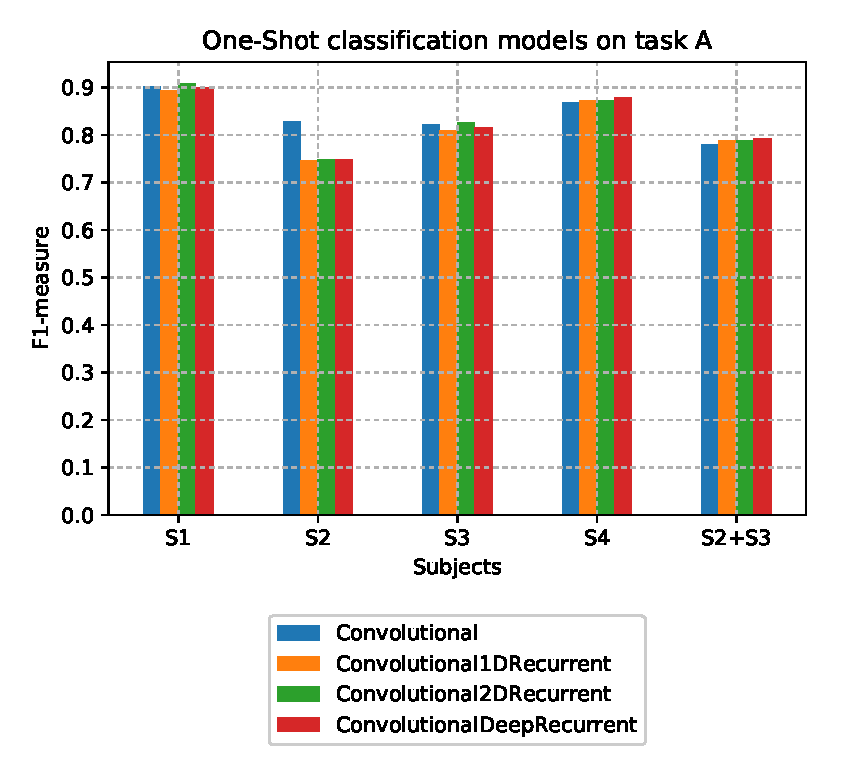
\includegraphics[scale=.4]{figure/A_models_nullclass}
	\caption{Task A : One-Shot Classification}
	\label{fig:A_os}
\end{figure}
\begin{figure}[t]
	\centering
	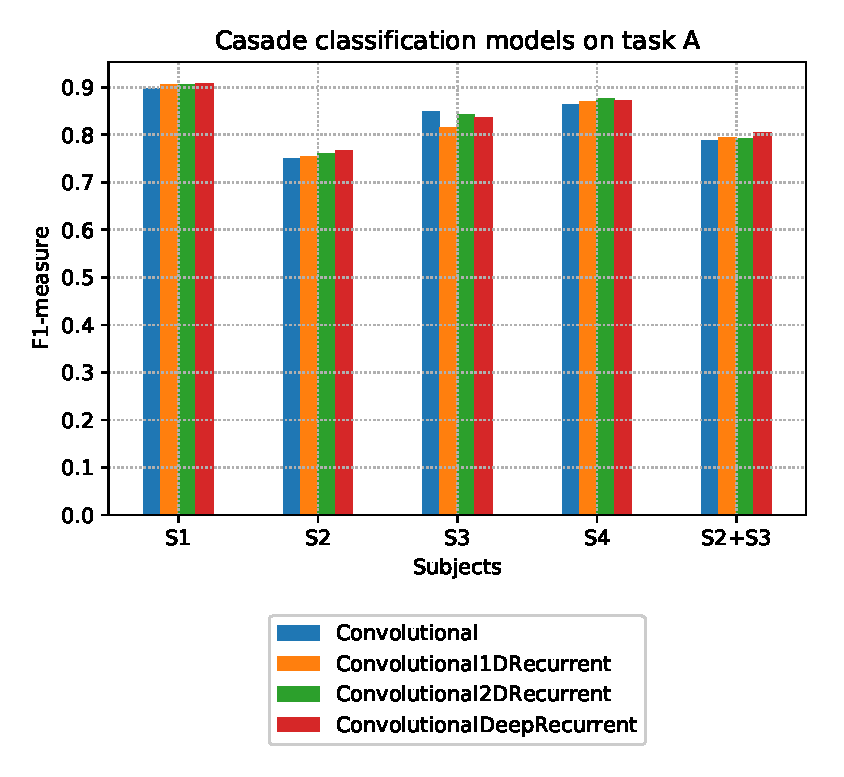
\includegraphics[scale=.4]{figure/A_models_cascade}
	\caption{Task A : Cascade Classification}
	\label{fig:A_casc}
\end{figure}

Since in \cite{Chavarriaga2013} results from the contributed methods have been compared to some baseline approaches, here we do the same by displaying only the best result for each type. In tables \ref{tab:res_A} and \ref{tab:res_B}
are reported respectively the results on task A and B, with and without the \textit{Null} class. Our results are taken then, for both tasks, from \textit{One-Shot Classification} and \textit{Activity Classification}, keeping only the best among the scores of the four models used.
We can see that sometimes our models perform better, particularly on \{S1, S3, S4\}, in other cases instead our score drops, as for \{S2\}, or is very similar to the others, as for \{[S2 S3]\}: it seems in fact that we have better results for those subjects for which contributed models in \cite{Chavarriaga2013} are worse, and viceversa. This is not though totally unexpected to us, since contributed models had to focus on \{S2, S3, [S2 S3]\}, while our attention has been more uniformly distributed.
What's surprising instead is what we obtained for S4, whose signals have been artificially affected by some rotational noise (task C in \cite{Chavarriaga2013}): we had good scores, compared to the others, but what's unexpected is that our performances for S4 are regularly better that the ones for S2.

In Figures \ref{fig:A_os} and \ref{fig:A_casc} we present the results regarding task A (modes of locomotion, high level movements) for each participant in the experiment: in those configurations we wanted to see if there was one architecture that evidently outperforms the others. As we can see, unfortunately, this is not the case since, among all the frameworks that we tested, the differences in terms of weighted $F_1$ measure are negligible: this suggests that the best model could be the simplest one, which is "Convolutional".
What we can clearly see instead are the variations among distinct subjects, since they are all investigated separately: $S1$ and $S4$ for example perform better in both the configurations, while $S2$ is typically the worst, as previously noticed.
The same considerations just discussed for task A are still valid for task B, as can be seen from the results showed in figures \ref{fig:B_os} and \ref{fig:B_casc}.

\begin{figure}[t]
	\centering
	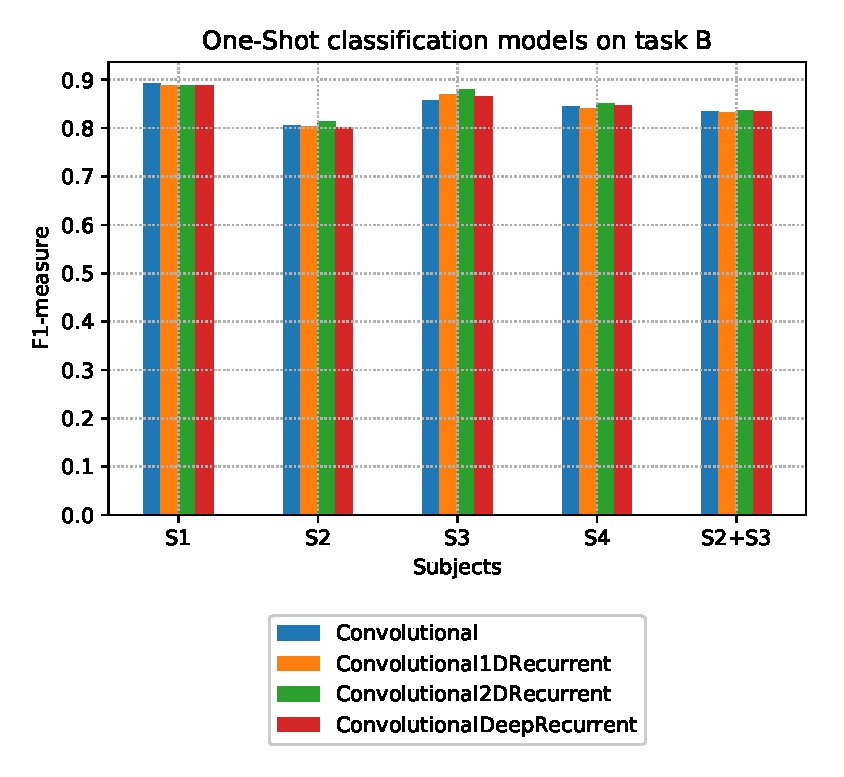
\includegraphics[scale=.4]{figure/B_models_nullclass}
	\caption{Task B : One-Shot Classification}
	\label{fig:B_os}
\end{figure}
\begin{figure}[t]
	\centering
	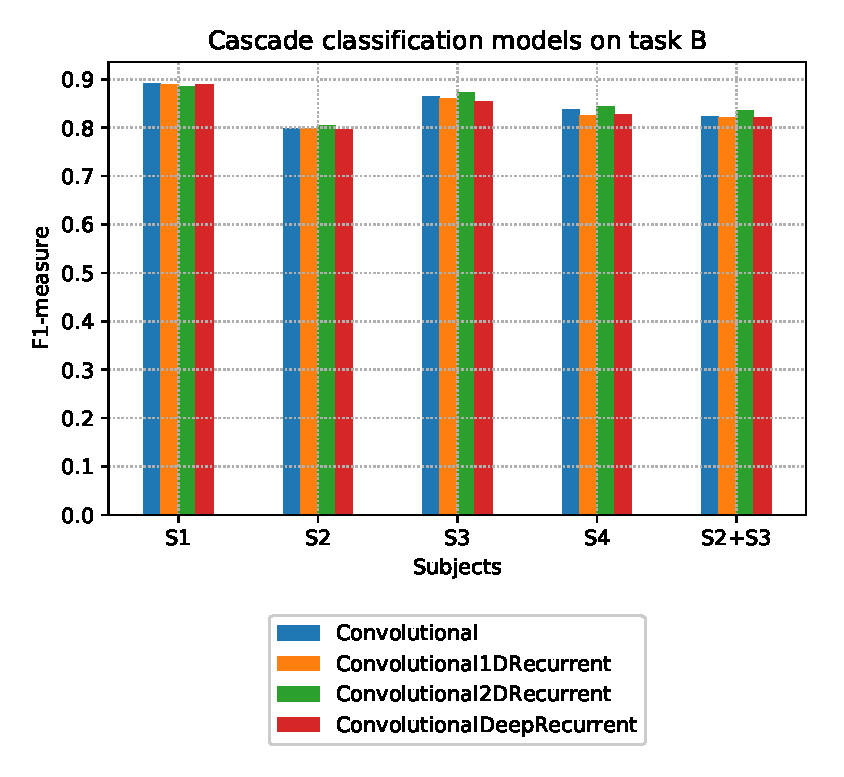
\includegraphics[scale=.4]{figure/B_models_cascade}
	\caption{Task B : Cascade Classification}
	\label{fig:B_casc}
\end{figure}

Focusing instead on the differences between the two pipelines, i.e. One-Shot and Cascade classifications, we see that also in this case that performances are very similar: splitting the pipeline into a detection and a classification gives a slight improvement on both tasks, in the order of $1\%$. For ease of assessment we report the results in figures \ref{fig:A_comp} and \ref{fig:B_comp}.
\begin{figure}[t]
	\centering
	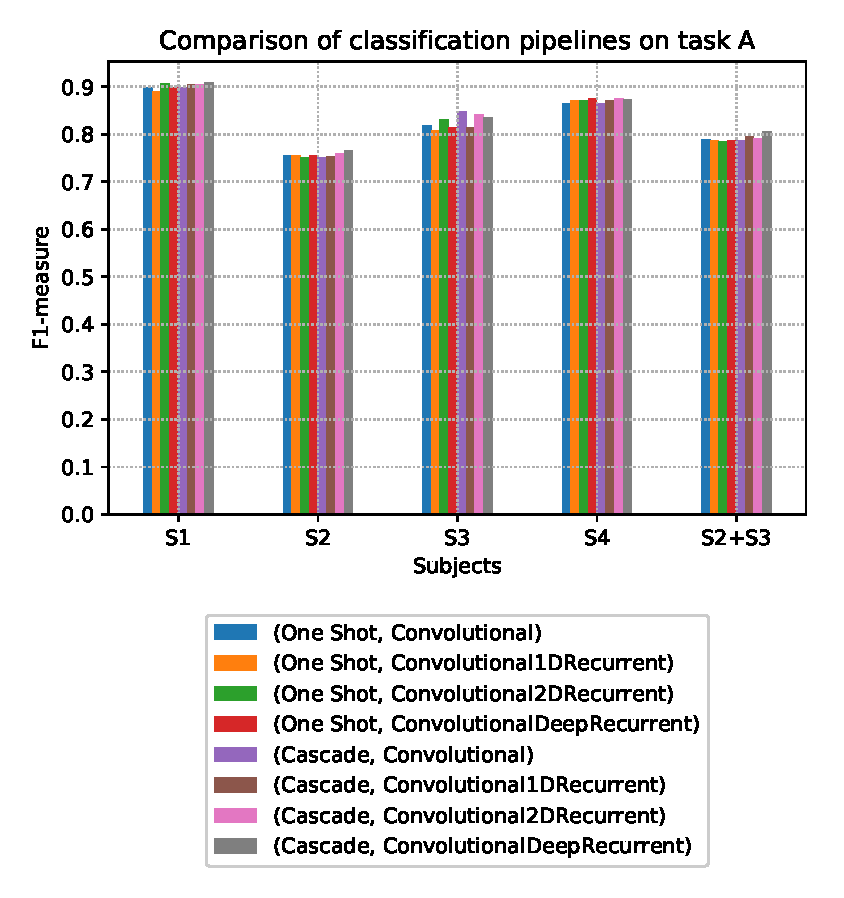
\includegraphics[scale=.6]{figure/A_pipeline_comparison}
	\caption{Task A : One-Shot and Cascade comparison}
	\label{fig:A_comp}
\end{figure}
\begin{figure}[t]
	\centering
	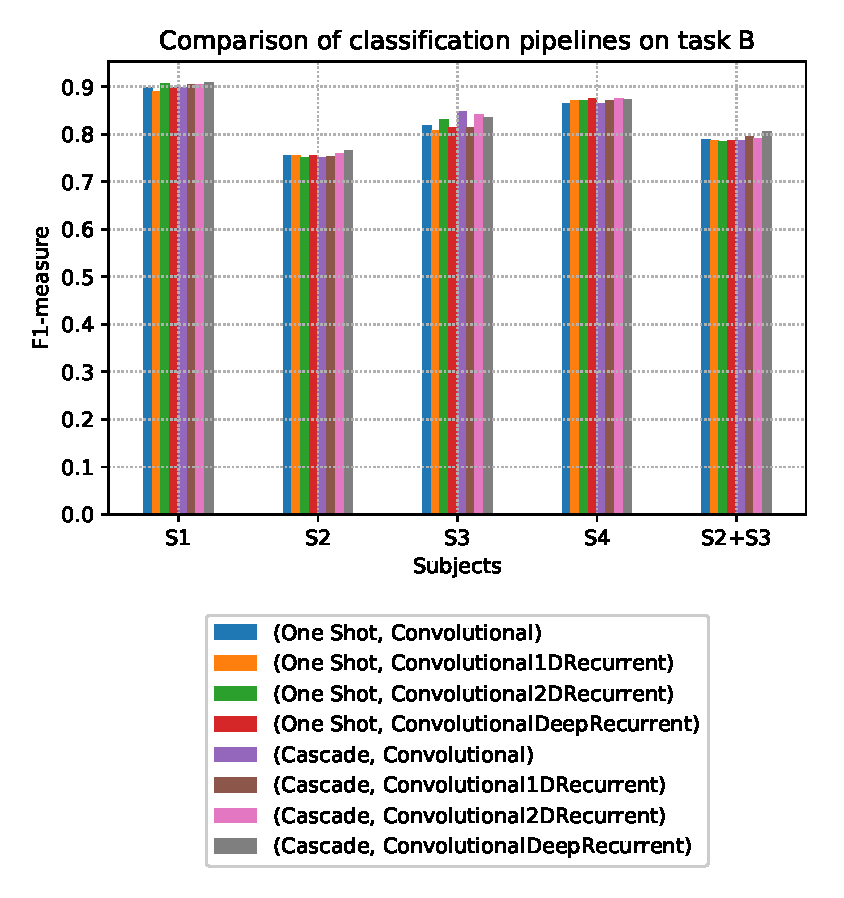
\includegraphics[scale=.6]{figure/B_pipeline_comparison}
	\caption{Task B : One-Shot and Cascade comparison}
	\label{fig:B_comp}
\end{figure}
Even though results for the Cascade classification don't seem to be that exciting, we can stay positive about them, keeping in mind that in our tests we always performed detection and classification with the same model, but there should be an increase in performances when using the best available model for each of the two tasks.

